\chapter[Evaluation]{Evaluation}
\label{sec:chapter5}

The evaluation of the developed privacy approach is made by means of two case studies. The aim of such case studies is to check if the stated objectives of this document (chapter \ref{sec:chapter3}) are satisfied. Specially, this chapter evaluates if software developers with few knowledge about privacy policies are able to handle the design of privacy-aware dataflow applications and if it is easy to reach a privacy-aware DIA from a non-privacy-aware streaming application.

In order to do that, first of all, the case studies are presented independently in two sections. Each section explains the context where the application is applied and which kind of statistics are computed. After that, the non-privacy-aware application is implemented explaining which kind of stereotypes are applied in the different sources, transformations and sinks as well as the required data types for each stream. Finally, the privacy approach is evaluated. In order to evaluate it, it is applied on the already developed non-privacy-aware application following two predefined steps:

\begin{enumerate}
\item Protected Streams Definition.
\item Privacy External Sources Definition.
\end{enumerate}

Finally, the UML class diagram developed with Papyrus is converted into the Flink codes by running a configuration in Eclipse which executes the developed Acceleo codes. The obtained Flink codes must be generated without errors independently of the implemented application.

In summary, this section faces the evaluation of the developed privacy approach and answers the following questions:

\begin{itemize}
\item Can software developers with few knowledge about privacy policies apply this approach?
\item Can software developers with few knowledge about Flink language apply this approach?
\item Is easily applicable the privacy approach once the non-privacy-aware DIA is already implemented?
%\item Are the Flink codes generated without errors independently of the implemented DIA?
\end{itemize}

\section{Great Seller Privacy Aware DIA}

In this section a DIA for an e-commerce company called Great Seller is implemented. This example implements the case study proposed in \cite{privacypoliciesarticle}. This proposed e-commerce DIA is able to compute real time statistics about the transactions generated by the consumers. Such statistics can be observed by some other companies that pay in order to have access to the information making that Great Seller acts as a data broker. In order to simplify the implementation, Great Seller is going to sell three different types of statistics:

\begin{itemize}

\item Statistic 1: the total amount of money that each consumer of Great Seller spend in the last 10 minutes.
\item Statistic 2: the number of transactions issued by each user in the last 10 minutes.
\item Statistic 3: the number of users who spent more than \euro{1000} in the last hour.

\end{itemize}

As any DIA, Great Seller generates such statistics by some transformations which are fed from a source and the generated information is stored into a sink which is accessible by the observer companies. Moreover, as Great Seller is producing three different types of statistics, its DIA requires three different sinks where the information should be stored. Due to the fact that Great Seller DIA is computing real time statistics about the transactions that are generated by the consumers of the company, only one source is required for the DIA model. Finally, one transformation is necessary for the computation of each statistic. In summary, Great Seller DIA requires one source, three transformations and three sinks for the design of its model.

The first step, after generating the Papyrus project (appendix \ref{sec:Appendix1}), is to define the model in the class diagram in order to specify that the application is going to be a Flink application. Then, first of all, we have to create a model node in the greatSellerApp.di file. This node is going to be called greatSeller as it is the object representing the whole application. Once the node is inserted, the properties of such node must be specified. More in detail, the Flink application stereotype has to be applied. In this case, the properties of the model has to be the default ones then nothing else must be done with this node. In the figure \ref{fig:Great Seller Data Types Package} can be seen how the stereotype has been applied to the model node.

\subsection{Great Seller Source}

In the implementation described along this section, Great Seller DIA is fed from a socket that reads from a text file where all the transactions generated by the consumers of Great Seller are stored. All the transactions are going to have the same predefined tuple structure 'transactionId,dataSubject,spentAmount,purchasedProduct'. This predefined structure is represented in the Great Seller DIA model by means of a data type called InputTransaction.

Regarding to the fields of such tuple, the transactionId field is an integer which varies from 1 to the number of generated transactions, such number can be 10, 100 or 1000. The dataSubject is the user who generates such tuple and, in this document, they possible data subjects are defined by a set of four names: Bob, Carlos, Elisabetta or Michele. The spentAmount is the price paid for the product that has been bought with the transaction and it is an integer with a low boundary of \euro{1} and an upper boundary of \euro{200}. Both boundaries are defined in this document and slightly vary from the boundaries proposed in \cite{privacypoliciesarticle} because they are considered too large for the scope of the privacy approach checker. Finally, the recipientId is the product bought with such transaction.

The steps that must be followed in order to add the data types that are requited to the application are the followings. First of all, a package node has to be inserted inside the Flink application model node. This package is called greatSellerDataTypes and a stereotype has to be applied as in the previous case. First of all, inside the properties window, in the profile field, the applied stereotype is defined. Inside this package all the datatypes that the application requires have to be inserted. The first data type is the InputTransactions which is composed of a transaction id (integer), a data subject (string), an amount (double) and a recipient id (string). The second data type is the IssuedTransactions which contains the data subject (string) and the number of transactions performed by such data subject which can be seen by means of the variable NTransactions (integer). The third data type is the SpentAmount which is composed of the data subject (string) and the total amount of money spent by the data subject which can be seen by means of the variable TotalAmount (double). Finally, the last data type is the NumberUsers which contains the number of users who spent more than 1000 dollars and it is represented by means of the variable NTopUsers (integer). Then, we need to insert one DataType node inside the package created in the previous step with each of these data types. Each data type can be seen as a tuple which is composed by several values. The name of the DataType node is going to be the same that the one corresponding to the tuple and each of the values that compose the tuple are going to be a property inside of the owned attributes that are specified in the UML field of the properties of each DataType node.In the table \ref{Great Seller Data Types} can be seen an abstract with all the data types required for this example. Moreover, in the figure \ref{fig:Great Seller Data Types Package} can be seen the package with all the data types of the application inserted in the application model with all the applied properties explained above.

\begin{table}[h!]
\centering
	\begin{tabular}{||c|c|c||} 
	\hline\hline
	Data Type & Property Name & Property Type \\ [1ex] 
	\hline\hline
	InputTransactions & transactionId & integer  \\
	& dataSubject & string  \\
	& amount & integer  \\
	& recipientId & string  \\
	\hline
	IssuedTransactions & dataSubject & string  \\
	& nTransactions & integer \\
	\hline
	SpentAmount & dataSubject & string  \\
	& totalAmount & integer \\
	\hline
	NumberUsers & NTopUsers & integer  \\
	\hline\hline
	\end{tabular}
\caption{Great Seller Data Types}
\label{Great Seller Data Types}
\end{table}

\begin{figure}
\centering
{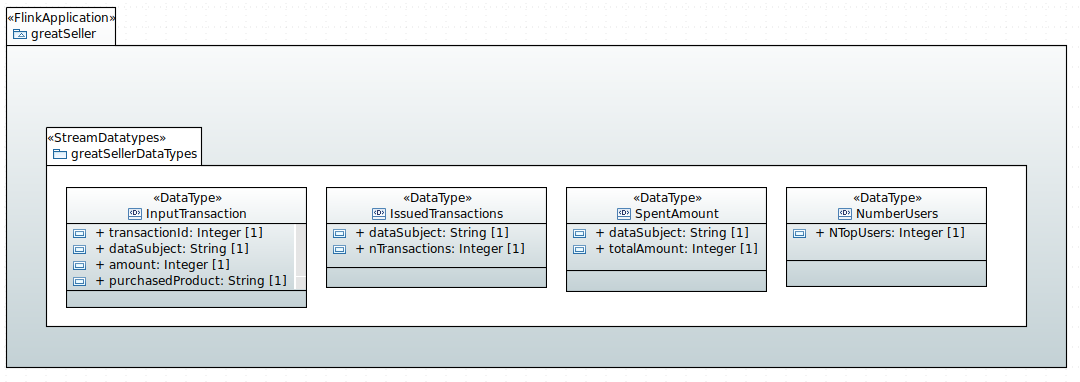
\includegraphics[scale=0.4]{./chapter4/greatSellerDiagram/greatSellerDataTypes.png}}
\caption{Great Seller Data Types Package}
\label{fig:Great Seller Data Types Package}
\end{figure}

It is important to remark that socket source introduces in the DIA a data stream of strings and the InputTransaction data type must be generated by means of a transformation which parses the string into the data type. This transformation is called TupleParser as it splits the incoming tuples, strings, into the InputTransaction data type.

The Great Seller stock is composed by means of 25 products. In order to simplify the implementation, each product is named by the word 'product' immediately followed by a number between 1 and 25 in order to specify the product referred in the stock. In the table \ref{Great Seller Stock} can be seen such stock.

\begin{table}[h!]
\centering
	\begin{tabular}{||c|c||} 
	\hline\hline
	Product & Price (\euro{}) \\ [1ex] 
	\hline\hline
	product1 & 196 \\ 
	\hline
	product2 & 36 \\ 
	\hline
	product3 & 179 \\ 
	\hline
	product4 & 17 \\ 
	\hline
	product5 & 120 \\ 
	\hline
	product6 & 187 \\ 
	\hline
	product7 & 139 \\ 
	\hline
	product8 & 52 \\ 
	\hline
	product9 & 160 \\ 
	\hline
	product10 & 110 \\ 
	\hline
	product11 & 113 \\ 
	\hline
	product12 & 67 \\ 
	\hline
	product13 & 100 \\ 
	\hline
	product14 & 125 \\ 
	\hline
	product15 & 192 \\ 
	\hline
	product16 & 115 \\ 
	\hline
	product17 & 113 \\ 
	\hline
	product18 & 98 \\ 
	\hline
	product19 & 113 \\ 
	\hline
	product20 & 185 \\ 
	\hline
	product21 & 143 \\ 
	\hline
	product22 & 18 \\ 
	\hline
	product23 & 194 \\ 
	\hline
	product24 & 41 \\ 
	\hline
	product25 & 26 \\ 
	\hline\hline
	\end{tabular}
\caption{Great Seller Stock}
\label{Great Seller Stock}
\end{table}

In order to generate this stock that feeds the Great Seller DIA, two Python codes have been developed. Furthermore, a Python server has been developed to input the transaction tuples to the dataflow application.

The first Python code (appendix \ref{sec:Appendix2Sec1}) builds a Python list which represents the Great Seller stock of 25 products and it assigns to each product a price. Each product is represented with a dictionary variable that contains a name variable and a price variable. The name variable is a string with the word 'product' immediately followed by an integer number from 1 to 25 which points to the product of the stock. The price is an integer number between \$1 and \$200 which is assigned randomly. Once the name and the price are assigned to the dictionary, the product is added to the stock list. Finally, the Great Seller stock list is saved in a binary shelf file in order to be accessible from the other Python code.

The second Python code (appendix \ref{sec:Appendix2Sec2}) generates the strings that represent the tuples produced by each consumer. In order to generate such tuples an integer number for the transactionId is assigned following an increasing numerical order from 1 to the maximum number of generated transactions which is input by command line to the code, it can be 10, 100 or 1000. After that, randomly, one of the four possible data subjects (Bob, Carlos, Elisabetta and Michele) and a product from the stock saved in the binary shelf file are assigned. Finally, each value is added to a string where each of these values are separated by a comma. The generated string represents the tuple produced by each consumer and it is written in the text file which is called from the Great Seller DIA in order to feed it.

Finally, the DIA inputs each of these strings into the DIA by means of a Python server (appendix \ref{sec:Appendix2Sec3}). This Python server introduces a non-parallel stream with the generated tuples (strings) and the stream is sent to the first transformation of the dataflow application.

\subsection{Great Seller Transformations}

The first transformation implemented in the application is the TupleParser. This transformation is a Map Transformation that is implemented in order to split the input strings supplied by the Python servers into the InputTransaction data type. This transformation takes advantage of the split Java method and it splits the strings by the comma generating the InputTransaction data type. The generated stream is sent to the OP1 and OP2 operators.

In order to compute each of the three statistics that Great Seller sells as data broker, the Great Seller DIA needs three transformations. Each of this transformations is the operator of each statistic. Thus, the operator one (OP1) computes the total amount of money spent by each user in the last 10 minutes. The second operator (OP2) computes the number of transactions issued by each user in the last 10 minutes. Finally, the operator three (OP3) computes the number of users who spent more than \euro{1000} in the last hour.

These transformations input a data stream with a set of tuples that all of them have identical structure. Thus, the first stream (S1) is composed of tuples of the kind InputTransaction. This stream is duplicated and it is sent to the operators OP1 and OP2. Moreover, as each operator works taking into account the data subject of each tuple, the stream S1 must be keyed by the data subject field of this first stream. Finally, as the operators have to compute the statistics taking into account only the tuples generated in the last 10 minutes, the stream S1 is windowed by a time window of 10 minutes.

The new data generated in the OP1 are represented in a new data type called SpentAmount and that is composed by two fields following the structure: 'dataSubject, totalAmount'. The SpentAmount tuples are collected in the stream S2 and they are keyed by the data subject field of such stream.

Finally, the data generated in the OP2, is collected in a new data type called IssuedTransaction whose structure is 'dataSubject, nTransactions'. This new stream (stream S3) is sent to the OP3. Moreover, this third stream is keyed by the data subject field of the stream and it is also windowed with a time window of one hour. The OP3 generates a randomly partitioned stream with an uniform distribution called stream S4 whose structure is: 'nTopUsers'.

\subsection{Great Seller Sinks}

Each of the tuples flowing through the streams S2, S3 and S4 are stored in a file. Such values are stored because the observer companies are able to access to the tuples. This is why, after each stream is generated (streams S2, S3 and S4), a file text sink is implemented. These file are going to be stored in the same location but with different names. The file resultsS2.txt stores the generated tuples in the stream S2; the file resultsS3.txt stores the values flowing through the stream S3 and the file resultsS4.txt stores the values of the stream S4.

This implementation is given due to the fact that each of the tuples generated by the operators are observable for the observer companies who buy them. Furthermore, such sinks allow to check if the transformations are well implemented by the designer of the DIA. In the figure \ref{fig:Great Seller StreamGen DIA} the developed model with StreamGen for the non-privacy-aware Great Seller DIA can be seen. In this figure is represented the same dataflow model that in the chapter \ref{sec:chapter3} but it is represented in Papyrus and it can be seen the applied stereotypes for the different sources, transformations and sinks in addition to the stream stereotypes.

\begin{figure}
\centering
{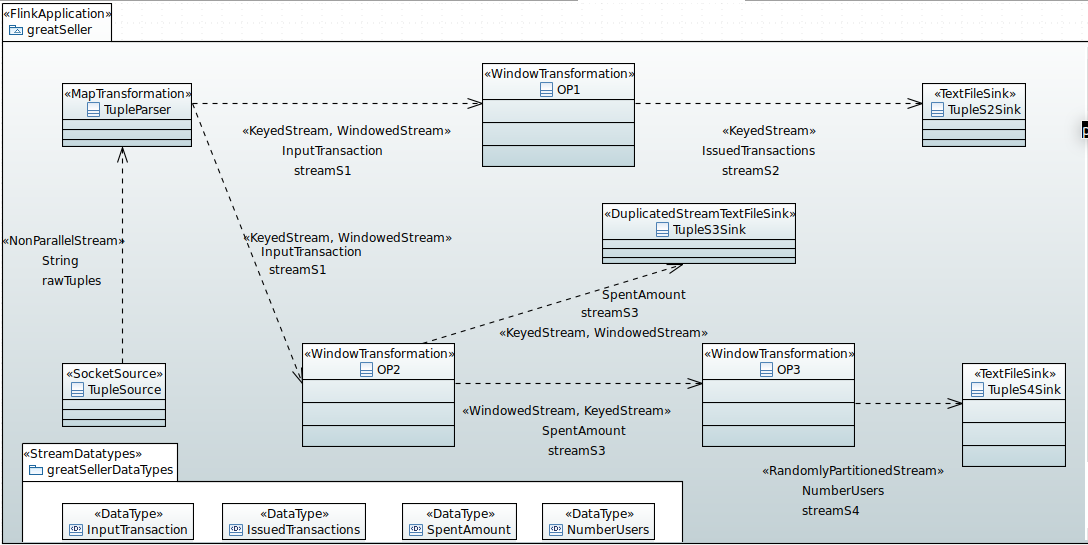
\includegraphics[scale=0.4]{./chapter3/greatSellerStreamGen.png}}
\caption{Great Seller StreamGen DIA}
\label{fig:Great Seller StreamGen DIA}
\end{figure}

\subsection{Great Seller Privacy Enforcement}

At this point, the non-privacy-aware dataflow application for the e-commerce company Great Seller is completed and the approach for the privacy-aware DIAs that is developed in this document must be applied in order to see if the previously stated objectives are met. The enforcement of the privacy model is made by means of two steps:

\begin{enumerate}
\item Protected Streams Definition
\item Privacy External Sources Definition
\end{enumerate}

\subsubsection{Protected Streams Definition}

Once the non-privacy-aware application is implemented, the privacy metamodel is applied. First of all, the streams that should be protected are specified. In the Great Seller application, such streams are streamS2 and streamS3. Then, the PrivacyProtectingStream stereotype is applied on both streams. However, streamS2 is protected by a VCP whilst streamS3 is protected by a DSEP. This means that the properties of the stereotypes are differents.

In the case of the streamS2 stereotype, as this stream is protected by a VCP, only such property must be true. In addition to this, the protectedStreamConf is specified according to the values that can be shown in the table \ref{PrivacyProtectingStream Great Seller StreamS2}. The timestampServerIp field of the protectedStreamConf is empty, this is why nothing is specified.

\begin{table}[h!]
\centering
	\begin{tabular}{||c|c|c||} 
	\hline\hline
	Property & Field Name & Field Value \\ [1ex] 
	\hline\hline
	protectedByVCP & - & true \\
	\hline
	protectedByDSEP & - & false \\
	\hline
	protectedStreamConf & monitoringActive & false \\
	 & timestampServerIp & \\
	 & timeStampServerPort & -1 \\
	 & topologyParallelism & 1 \\
	 & simulateRealisticScenario & false \\
	 & allowedLateness & 0 \\
	 & logDir & /home/cablan/Desktop/thesis/conf/ \\
	\hline\hline
	\end{tabular}
\caption{PrivacyProtectingStream Great Seller StreamS2}
\label{PrivacyProtectingStream Great Seller StreamS2}
\end{table}

StreamS3 is specified in a similar way, in this case the protectedStreamConf is exactly the same but the protectedByVCP property is false and the protectedByDSEP is true. In the table \ref{PrivacyProtectingStream Great Seller StreamS3} can be seen the specified. As in the other case, the timestampServerIp field is empty because no value is specified there.

\begin{table}[h!]
\centering
	\begin{tabular}{||c|c|c||} 
	\hline\hline
	Property & Field Name & Field Value \\ [1ex] 
	\hline\hline
	protectedByVCP & - & false \\
	\hline
	protectedByDSEP & - & true \\
	\hline
	protectedStreamConf & monitoringActive & false \\
	 & timestampServerIp & \\
	 & timeStampServerPort & -1 \\
	 & topologyParallelism & 1 \\
	 & simulateRealisticScenario & false \\
	 & allowedLateness & 0 \\
	 & logDir & /home/cablan/Desktop/thesis/conf/ \\
	\hline\hline
	\end{tabular}
\caption{PrivacyProtectingStream Great Seller StreamS3}
\label{PrivacyProtectingStream Great Seller StreamS3}
\end{table}

In the figure \ref{fig:Great Seller Privacy Aware StreamGen DIA} can be seen how looks the application after defining the streams that are protected. This figure represents the same model that the one that is shown in \ref{fig:Great Seller StreamGen DIA} but adding the PrivacyProtectingStream stereotype on those streams that are protected.

\begin{figure}
\centering
{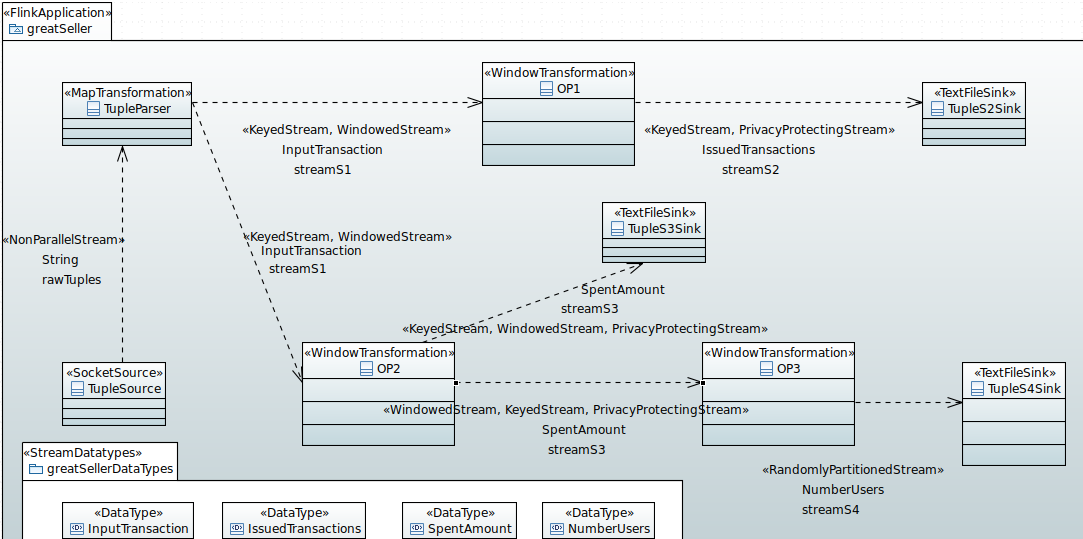
\includegraphics[scale=0.4]{./chapter5/privacyGreatSellerApp.png}}
\caption{Great Seller Privacy Aware StreamGen DIA}
\label{fig:Great Seller Privacy Aware StreamGen DIA}
\end{figure}

\subsubsection{Privacy External Sources Definition}

Once the privacy streams have been defined, the second step is to define the SCV source and the privacy rules source. The privacy rules source have only one choice; however, the SCV source can be defined in several ways. In this example, as the input is working with sockets, the socket source is defined for this purpose.

But before introducing the classes of the sources, the PrivacyPolicyPackage stereotype must be defined in a new package in order to make more intuitive the approach to the DIA developer. In order to do this, a new package node is introduced in the application model node and the stereotype PrivacyPolicyPackage is applied in such new package that is called PrivacyPolicyInputs. Once the package is introduced into the model, the SCV source is defined. In order to do this, a new class is introduced inside the package called PrivacyPolicyInputs and the PrivContSocketSource stereotype is applied on it. Such new class is called StaticContextVariablesSource and their properties are filled with the values localhost (host, string) and 9998 (port, integer). Finally, another new class is introduced in the package. In this case, it is called PrivacyPolicySource and the PrivPolYamlFileSource stereotype is applied on it. This stereotype contains only one property (pathToFile) that must be filled. In this case, it is filled with the value /home/cablan/Desktop/thesisFiles/config/privacy-config.yml that is the path where the YAML file is located.

In the figure \ref{fig:Great Seller Privacy Policy Package} can be seen the introduced package with the PrivacyPolicyPackage stereotype applied on it and two nested classes that represent the privacy sources with their applied stereotypes, PrivContSocketSource and PrivPolYamlFileSource. As it can be seen there, the package makes intuitive the way in which the privacy external sources are introduced to the dataflow application and the sources classes follow the same approach that any StreamGen source. 

\begin{figure}
\centering
{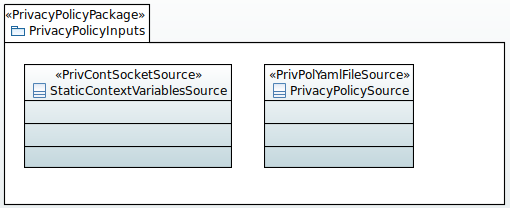
\includegraphics[scale=0.7]{./chapter5/privacyPolicyPackage.png}}
\caption{Great Seller Privacy Policy Package}
\label{fig:Great Seller Privacy Policy Package}
\end{figure}

At this point, the privacy-aware DIA is implemented and the configuration is run in order to generate the Java codes of the application. In the appendix \ref{sec:Appendix3} can be seen how to run such configuration.

\subsection{Great Seller DIA Limitations}

After developing this DIA, some limitations are identified relative to the current development of StreamGen. The first limitation is the number of servers that can be connected directly to a Map Transformation. In this example, it is supposed that the users send the transactions by means of a server to the target DIA. This server is the same for all the users who are using Great Seller DIA. At this point, a casuistry is proposed. This is the case of a DIA involved in an industry 4.0 application where the owner of the factory cannot afford to invest in a server for the DIA and all the machines generating datasets must be connected directly to the DIA by means of the factory net.

The second limitation that is extracted is that StreamGen does not allow to generate float or double data types. In this example, Great Seller is working with a stock where all the products have integer prices but should be necessary a DIA which allows, among the language, to declare float or double values.

In the following example, both casuistry are fixed and the privacy model is applied to check its behavior.

\section{Cool Analyst Privacy Aware DIA}

In addition to Great Seller, another DIA is developed with StreamGen in order to check more in detail the developed approach for the privacy-aware DIAs. This is the case of Cool Analyst, a DIA which is able to compute some statistics from the temperatures measured in two different refrigeration chambers of a panettone factory called Panettone 4.0. These measurements are going to be stored in a CSV file in order to be accessible by the manager of the industrial plant to see if any problem has been produced in the yeast fermentation. This application is going to compute four statistics in two different operators:

\begin{itemize}
\item Operator 1: the maximum, the minimum and the average temperature of each chamber during the last 5 minutes.
\item Operator 2: the prediction of the temperature for the next 10 minutes.
\item Operator 3: the filtered data between a range which have no null value and no null id.
\end{itemize}

Cool Analyst DIA is going to require two socket sources, one for each of the industrial chambers, two transformations in order to compute each of the operators specified before and two sinks where the CSV files with each of the results of the operators can be stored. For the development of the prediction operator, as its development is out of this document, it is taken from an already working transformation for such purpose.

Following the Great Seller approach, before generating the dataflow application, the first step is to create the Papyrus project according to the appendix \ref{sec:Appendix1}. After that, the application model is introduced in the Papyrus project. In order to do this, a model node is defined in Papyrus and the steotype FlinkApplication is applied on it. As in the previous example, the default properties for such stereotype are the final ones, then, they must not be modified. In the figure \ref{fig:Cool Analyst Data Types Package} can be seen the Papyrus model and the applied stereotype for the Cool Analyst application model.

\subsection{Cool Analyst Sources}

Panettone 4.0 is using temperature digital sensors in each of its two chambers where yeasts are fermented. These sensors are connected to the net of the factory and are sending the measured values directly to the Cool Analyst DIA with a 1 second sample frequency.

This two chambers need to control the temperature of the room in order to allow the correct fermentation of the yeasts. The role of the first chamber is to make the primary fermentation in the production process of the Panettone 4.0 factory. This fermentation is also known as bulk fermentation. On the other hand, the role of the second camera is to make the secondary fermentation which is also known as proofing. More information can be read about the fermentation of the years and how to control the temperature during its production in \cite{yeastfermentation}. The conclusions that are extracted from \cite{yeastfermentation}, and that are useful for our purpose, are that the bulk fermentation must have the temperatures of the room in the range [20, 24] Celsius whilst the secondary fermentation must have an environment with temperatures in the range [22, 29] Celsius. This is why Cool Analyst requires two socket sources connected to the port and to the host of each of the chambers.

The two sockets send a tuple with the chamber identifier (room1 or room2) and the temperature of the chamber in a string separating both values by a comma. This string, as happens in the Great Seller example, is sent to a parser which generates a data type and, then, Cool Analyst works with several data types that must be defined in a package according to the StreamGen behavior. In order to do this, a package node is introduced into the model node and it is called coolAnalystDataTypes. After that, the StreamDatatypes stereotype is applied on the package and all the data types required by the DIA are defined. The first data type is the roomTemp data type. It is composed of two different values: roomId (string) that is the identifier of the chamber and roomTemp (double) which is the current temperature of the chamber. The second required data type is the roomStatistics data type which is composed of four values: roomId (string), maxTemp (double), minTemp (double) and avgTemp (double). The three last values of the roomStatistics data type (maxTemp, minTemp and avgTemp) are the maximum, minimum and average computed values of the chamber identified with the roomId string. Finally, the last requited data type for the Cool Analyst DIA is the tempPred which is a prediction of the chambers for the following ten seconds. This data type is composed of the values roomId (string) and predTemp (double) which are the predicted temperature of the room identified by the roomId string. For each of the three data types required by the Cool Analyst DIA, a Data Type node is inserted in the package called coolAnalystDataTypes and a property for each of the values that compose the data type are inserted as an owned attribute of the data type. In the table \ref{Cool Analyst Data Types} can be seen an abstract with all the data types required by the dataflow application. Furthermore, in the figure \ref{fig:Cool Analyst Data Types Package} can be seen the package with all the data types of the Cool Analyst application, explained above, inserted in the application model according to the StreamGen approach.

\begin{table}[h!]
\centering
	\begin{tabular}{||c|c|c||} 
	\hline\hline
	Data Type & Property Name & Property Type \\ [1ex] 
	\hline\hline
	roomTemp & roomId & string  \\
	& roomTemp & double  \\
	\hline
	roomStatistics & roomId & string  \\
	& maxTemp & double \\
	& minTemp & double  \\
	& avgTemp & double \\
	\hline
	tempPred & roomId & string  \\
	& predTemp & double \\
	\hline\hline
	\end{tabular}
\caption{Cool Analyst Data Types}
\label{Cool Analyst Data Types}
\end{table}

\begin{figure}
\centering
{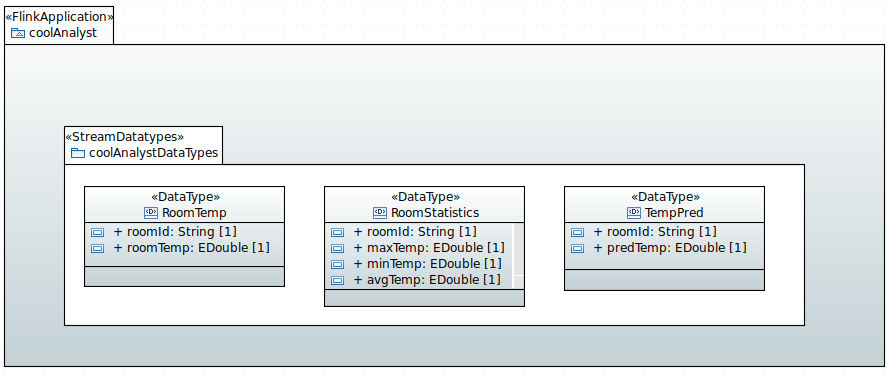
\includegraphics[scale=0.7]{./chapter5/coolAnalystDataTypes.png}}
\caption{Cool Analyst Data Types Package}
\label{fig:Cool Analyst Data Types Package}
\end{figure}

Also it is important to remark how the temperatures of the chambers are simulated. For such purpose a python code has been developed for each of the chambers (appendices \ref{sec:Appendix2Sec4} and \ref{sec:Appendix2Sec5}). These models take as target temperature, the average temperature of each of the ranges. This temperature is supposed to be maintained during ten seconds. Then, randomly, the program generates an increasing or decreasing sine function with a frequency of 1/16 Hz for the lower range and with a frequency of 1/28 Hz for the upper range. The lower range is considered from the lower boundary of each of the ranges of temperature that the chambers can admit ([22, 29] Celsius in the chamber one and [20, 24] Celsius in the chamber two) until the average temperature and the upper range from the average temperature until the upper boundary of the ranges. In the figures \ref{fig:Temperature Chamber 1 Model} and \ref{fig:Temperature Chamber 2 Model} can be seen both models. The simulation is built for one hundred temperature values.

\begin{figure}
\centering
{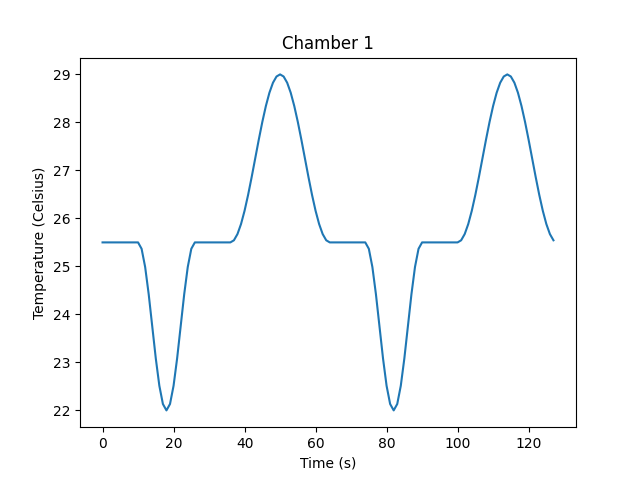
\includegraphics[scale=0.7]{./chapter3/room1TempModel.png}}
\caption{Temperature Chamber 1 Model}
\label{fig:Temperature Chamber 1 Model}
\end{figure}

\begin{figure}
\centering
{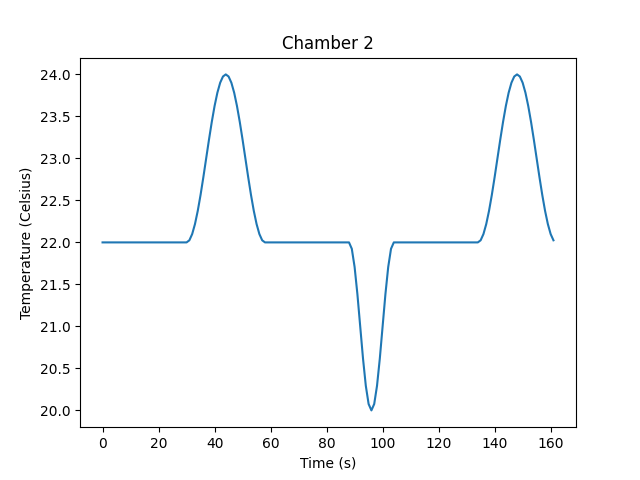
\includegraphics[scale=0.7]{./chapter3/room2TempModel.png}}
\caption{Temperature Chamber 2 Model}
\label{fig:Temperature Chamber 2 Model}
\end{figure}

Finally, these two models are saved in a TXT file which is going to be read from two Python servers (appendices {sec:Appendix2Sec6} and {sec:Appendix2Sec7}) that are developed in order to simulate the chambers working independently. These servers read one value each second during the period that the simulation lasts. This generates that the socket sending the values from the chamber one stops earlier than the other socket. This model design allows to proof the right behavior of the whole application, allowing to see what would happen if, suddenly, the sensors are disconnected.

\subsection{Cool Analyst Transformations}

The values read from the TXT file are sent in a string which has to be parsed in order to generate the data types that are used in the DIA. The strings contain the roomId followed by the temperature and both values are separated by means of a comma. This is why, first of all a NMap transformation called generateFlinkCoMapTransformation is developed. In order to do this, in the generateFlinkTransformations.mtl file, the existing but not developed generateFlinkCoMapTransformation is written taking as approach the transformations called generateFlinkCoFlatmapTransformation and generateFlinkMapTransformation. In the following code can be seen the written Acceleo code.

\lstinputlisting{./chapters/filesAppen/nMapTrans}

This NMap transformation inputs the two streams with the strings sent by the room servers and the incoming strings are parsed into a roomTemp data type which is composed of two properties: roomId (string) and roomTemp(double). Furthermore, in order to introduce double values from the Papyrus model by means of StreamGen, the generateDataTypes.mtl file is slightly modified. The modification is made considering the code previously developed for the Long values. Then, every time that a property name is EDouble, it is substitute by Double. In the figure following code can be seen one of the added pieces of code to the file and how this approach follows the Long approach. Moreover, this piece of code is added several times, as many times as necessary.

\lstinputlisting{./chapters/filesAppen/doubleDT}

Once the roomTemp data type is generated, a stream is sent to a window transformation called RoomStatistics. In this transformation all the computations explained previously in the operator one are calculated (maximum temperature, minimum temperature and average temperature). This transformation generates a new data type called roomStatistics. Then, the stream with the roomStatistics data types is sent to the TemperaturePredictor transformation. This window transformation computes the operations described in the operator two and generates the tempPred data type. The last operator takes the stream with the roomTemp data type from the RoomStatistics transformation and, by means of a filter transformation called CleanRawData, checks that there is no temperature with a value below -9999 neither 9999. Moreover, this transformation checks that the temperature has a value and that value is referenced to a room identifier.

\subsection{Cool Analyst Sinks}

Finally, the data types generates in the RoomStatistics, in the TemperaturePredictor and in the CleanRawData transformations are stored each one in its sink. Cool Analyst uses CSV sinks as this kind of files are commonly used by engineers who work in the factories. In order to do this, the output stream from the RoomStatistics transformation is sent to StatisticsSink where is specified the path of the generated file, the output stream from the TemperaturePredictor transformation is sent to PredictorSink where the path of the second output file is specified and the same proceadure is done with the third operator CleanRawData and its sink CleanDataSink.

In the figure \ref{fig:Cool Analyst StreamGen DIA} can be seen the Cool Analyst StreamGen DIA explained above which is the non-privacy-aware application of the Cool Analyst DIA.

\begin{figure}
\centering
{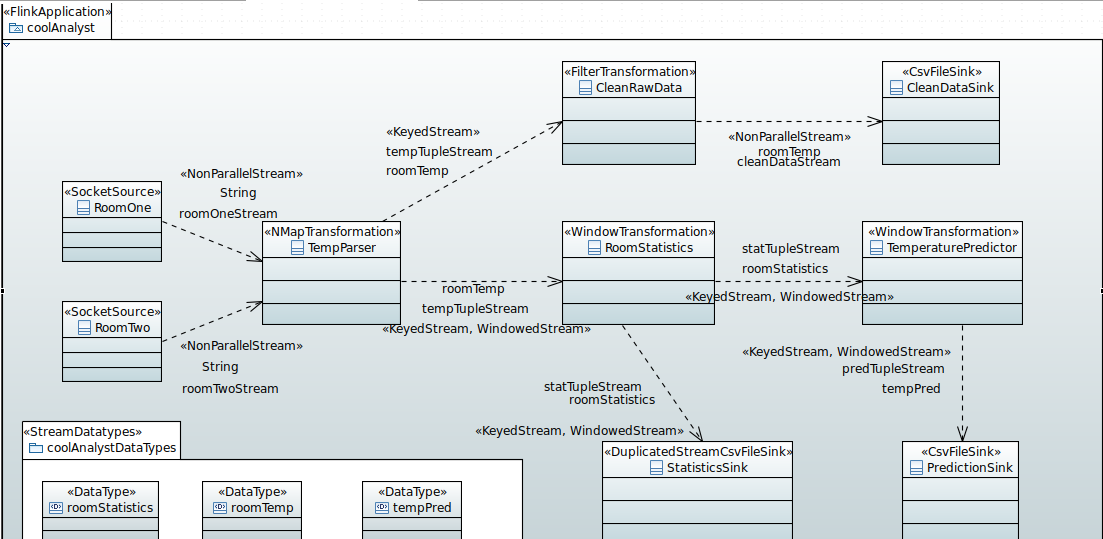
\includegraphics[scale=0.4]{./chapter3/coolAnalystStreamGen.png}}
\caption{Cool Analyst StreamGen DIA}
\label{fig:Cool Analyst StreamGen DIA}
\end{figure}

\subsection{Cool Analyst Privacy Enforcement}

At this points, the privacy approach for dataflow applications is applied to the already developed non-privacy-aware DIA model by defining the two already known steps. This example allows to check what happens with the developed approach for privacy-aware dataflow applications when a transformation generates a stream that is required to be protected partially, depending on the destination transformation.

\subsubsection{Protected Streams Definition}

In this DIA a DSEP is required in order to avoid tuples coming from the first chamber to be considered in the computation of the RoomStatistics transformation. From the designer perspective, no more information is required in order to define the characteristics of the protected stream. This is why only one stream requires to be protected by privacy policies.

In order to do this, the PrivacyProtectingStream stereotype is applied in the stream known as tempTupleStream flowing from the TempParser transformation to the RoomStatistics transformation. Once the stereotype is applied, the properties for such stereotype are defined. In this case, the stream is protected by a DSEP (protectedByDSEP is true) but it is not protected by any VCP (protectedByVCP is false). Moreover, protectedStreamConf data type is defined with the same values that the protected streams in the Great Seller example were designed. In the table \ref{PrivacyProtectingStream Cool Analist TempTupleStream} can be seen how are defined all these values.

\begin{table}[h!]
\centering
	\begin{tabular}{||c|c|c||} 
	\hline\hline
	Property & Field Name & Field Value \\ [1ex] 
	\hline\hline
	protectedByVCP & - & false \\
	\hline
	protectedByDSEP & - & true \\
	\hline
	protectedStreamConf & monitoringActive & false \\
	 & timestampServerIp & \\
	 & timeStampServerPort & -1 \\
	 & topologyParallelism & 1 \\
	 & simulateRealisticScenario & false \\
	 & allowedLateness & 0 \\
	 & logDir & /home/cablan/Desktop/thesis/conf/ \\
	\hline\hline
	\end{tabular}
\caption{PrivacyProtectingStream Cool Analist TempTupleStream}
\label{PrivacyProtectingStream Cool Analist TempTupleStream}
\end{table}

The value for the timestampServerIp is empty because, as in the previous example, it is defined to nothing. All these values can be modified but they are considered as the default values for any protected stream.

In the figure \ref{fig:Cool Analyst Privacy Aware StreamGen DIA} can be seen the applied stereotype in the non-privacy-aware application in order to defined which streams are protected.

\begin{figure}
\centering
{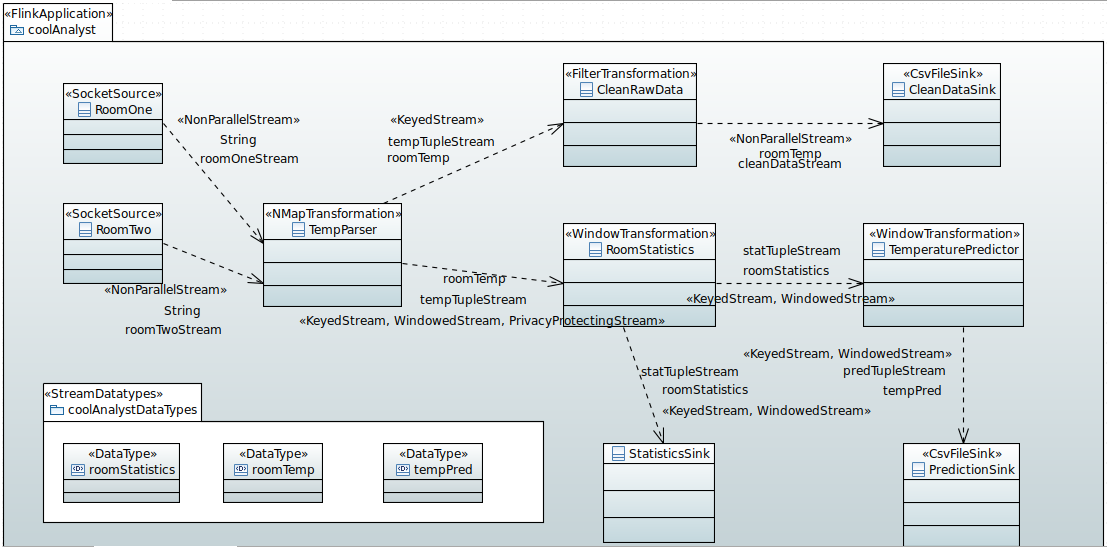
\includegraphics[scale=0.4]{./chapter5/coolAnalystPrivacyDIA.png}}
\caption{Cool Analyst Privacy Aware StreamGen DIA}
\label{fig:Cool Analyst Privacy Aware StreamGen DIA}
\end{figure}

\subsubsection{Privacy External Sources Definition}

After defining the protected streams, the external privacy sources are introduced. In this case, the predefined DSEP must be applied every time that an employee who is not the manager of the Panettone 4.0 factory tries to see the statistics of the first chamber. Then, a TXT file with all the employee identifiers and assuming that they try to access with analytical purposes is created and accessed by the SCV source.

In order to implement this, first of all, a package node called ExternalPrivacySources is introduced in the application model and the PrivacyPolicyPackage stereotype is applied on it in order to make more intuitive how to introduce the SCV source and the privacy rules source.

After that, a class node called SCVSource is introduced in the ExternalPrivacySources package and the PrivContTextFileSource stereotype is applied on it. This stereotype requires to define the pathToFile (string) property, in the table \ref{Cool Analist External Sources Properties} can be seen such path. Moreover, in the table \ref{Cool Analist SCV Text File} can be seen the content of the text file.

Once the SCV source is completely defined, the privacy rules source is introduced. For such purpose, a class node called PrivacyRulesSource is introduced in the ExternalPrivacySources package. In this class the PrivPolYamlFileSource is applied and its property, pathToFile (string), is defined according to the table \ref{Cool Analist External Sources Properties}.

\begin{table}[h!]
\centering
	\begin{tabular}{||c|c|c||} 
	\hline\hline
	Class & Property Name & Property Value \\ [1ex] 
	\hline\hline
	SCVSource & pathToFile & /home/cablan/Desktop/thesis/conf/ \\
	\hline
	PrivacyRulesSource & pathToFile & /home/cablan/Desktop/thesis/conf/ \\
	\hline\hline
	\end{tabular}
\caption{Cool Analist External Sources Properties}
\label{Cool Analist External Sources Properties}
\end{table}

\begin{table}[h!]
\centering
	\begin{tabular}{||c|c|c||} 
	\hline\hline
	Observer Identifier & Purpose & Role \\ [1ex] 
	\hline\hline
	employee1 & analytics & employee \\
	\hline
	employee2 & analytics & employee \\
	\hline
	employee3 & analytics & employee \\
	\hline\hline
	\end{tabular}
\caption{Cool Analist SCV Text File}
\label{Cool Analist SCV Text File}
\end{table}

At this point, the privacy-aware DIA is implemented and the configuration is run in order to generate the Java codes of the application. In the appendix \ref{sec:Appendix3} can be seen how to run such configuration.

\section{Discussion}

Great Seller and Cool Analyst are two DIA developed in this document in order to evaluate the privacy approach explained in chapter \ref{sec:chapter4}. The aim of this evaluation is to answer some previously stated questions:

\begin{itemize}
\item Can software developers with few knowledge about privacy policies apply this approach?
\end{itemize}

As it can be seen in both examples, software developers just need to know if a stream is protected by VCPs and DSEPs independently of the number of policies that are applied on them. Moreover, software developers apply the privacy policies by adding a stereotype to the stream that must be protected in the same way that a windowed or keyed stream is specified.

\begin{itemize}
\item Can software developers with few knowledge about Flink language apply this approach?
\end{itemize}

Due to the fact that the approach imports an already developed library with a predefined structure, the generated Flink codes by means of Acceleo follow the same structure independently of the implemented DIA. This is why, codes must not be modified by software developers and, then, it is not required that they need any knowledge about the target language, in this case Flink language.

\begin{itemize}
\item Is easily applicable the privacy approach once the non-privacy-aware DIA is already implemented?
\end{itemize}

In both case studies developed in this chapter, the privacy-aware DIA is reached only by following two simple steps (protected streams definition and privacy external sources definition) once the non-privacy-aware application is already implemented. Moreover, both steps are defined considering the already existing approach to introduce data types by means of a package and by applying a stereotype in those streams that must be protected.

In summary, with this two case studies can be seen how the objectives stated in chapter \ref{sec:chapter3} are satisfied.

